\chapter{Teorija}
Šajā nodaļā tiek aprakstīta VSRC X-joslas raidzutveršanas sistēma, VSRC augstas jaudas pastiprinātājs, dziļā kosmosa misiju spektra sadalījums, VSRC dotā specifikācija darba punkta iestatīšanai jaudas pastiprinātājam, ieskats RF jaudas pastiprinātāju vadības sistēmās un pieejamās integrālās shēmas, virziena nozarotāja darbības princips, jaudas detektori, diferenciālā mērīšanas metode un S-parametri.

\section{RT-16 X-joslas raiduztverošās sistēmas pārskats}
Att 1.1. tiek parādīta X-joslas pārskats RT-16 radioteleskopam. Sistēmas vadība tiek veikta ar operatora jeb kontroles datoru, kas vada Cortex modemu \cite{cortex}, frekvenču lejuppārveidotāju un augšuppārveidotāju \cite{up_down_converters}, LNA un HPA. Cortex modēms paredzēts datu modulēšanai un demodulēšanai no satelīta. Frekvenču lejup un augšup pārveidotājs nepieciešams, lai varētu modulēto signālu pārnest uz nepieciešamo nesējfrekvenci noteiktam satelītam. HPA pastiprina modulēto signālu līdz 100 W (+50 dBm), lai palielinātu pārraides attālumu. HPA bloka pārraides jaudu noteica SSC. LNA nepieciešams, lai uzlabotu uztvertā signāla SNR un lai Cortex varētu to veiksmīgi demodulēt. Dipleksers un paraboliskā antena paredzēti signāla uztveršanai un pilna dupleksa komunikācijas nodrošināšanai.
\begin{figure}[H]
	\centering
    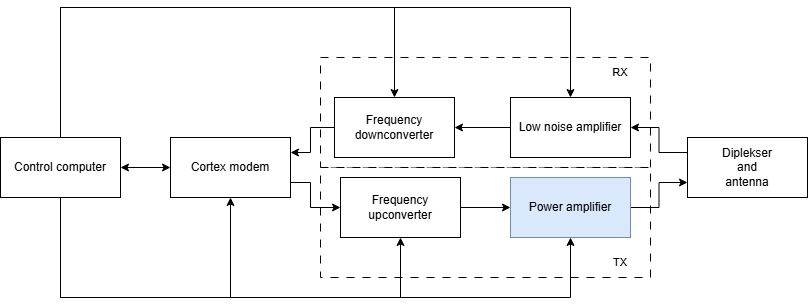
\includegraphics[width=\textwidth]{pictures/rt-16_x_diagram.jpg}\hspace{1cm}
    \caption{RT-16 X-joslas raiduztvērēja vispārīga bloka diagramma}
\end{figure}
Turpmāk darbā tiek apskatīts tikai augstas jaudas pastiprinātājs, kur daļa no tā tiek izstrādāta šī bakalaura ietvaros.
\section{Augstas jaudas pastiprinātājs}
No frekvenču augšuppārveidotāja signāla pievade notiek caur SMA konektoru, tad signāls tiek padots uz priekšpastiprinātāju KU PA 640720-10A\cite{pre_amplifier}, lai pastiprinātu ienākošo signālu par 30 dB. Priekšpastiprinātājam tiek nodrošināta jauda ar industriālā tipa barošanas avotu no 230 VAC uz 12 VDC. Tad +30 dBm signāls tiek nodots sadalītājam, kur uz katru kanālu tiek padota puse no ienākošās jaudas, kas ienākošo +27 dBm signālu pastiprina vēl par \textasciitilde19 dB katrs, kur tālāk +46 dBm signāls no katra kanāla tiek padots uz summatoru, pēc kā ir +\textasciitilde49 dBm, kur signāls tiek nogādāts uz nozarotāju, kur tālāk nogādāts N-tipa konektoram. Pie nozarotāja tiek pievienota jaudas monitorēšanas sistēma, lai noteiktu izstaroto un atstaroto jaudu. Darba punkta iestatīšanas un atiestatīšanas sistēma vajadzīga, lai nodrošinātu sistēmas drošu darbību.
HPA ir balstīts uz Qorvo QPM1017, kas darbojas vajadzīgajā augšupsaites joslā 7.145 līdz 7.235 GHz. Viens HPA modulis spēj nodrošināt līdz +50 dBm izejas jaudu ar 30… 40\% efektivitāti pie 7,2 GHz. Lai gan teorētiski viena moduļa izejas jauda ir +50 dBm, darba vadītājs nolēma apvienot divus QPM1017, kas ļautu katrai atsevišķai ierīcei darboties ar pusi no tās maksimālās jaudas, tādējādi uzlabojot termālo veiktspēju.
\begin{figure}[H]
	\centering
    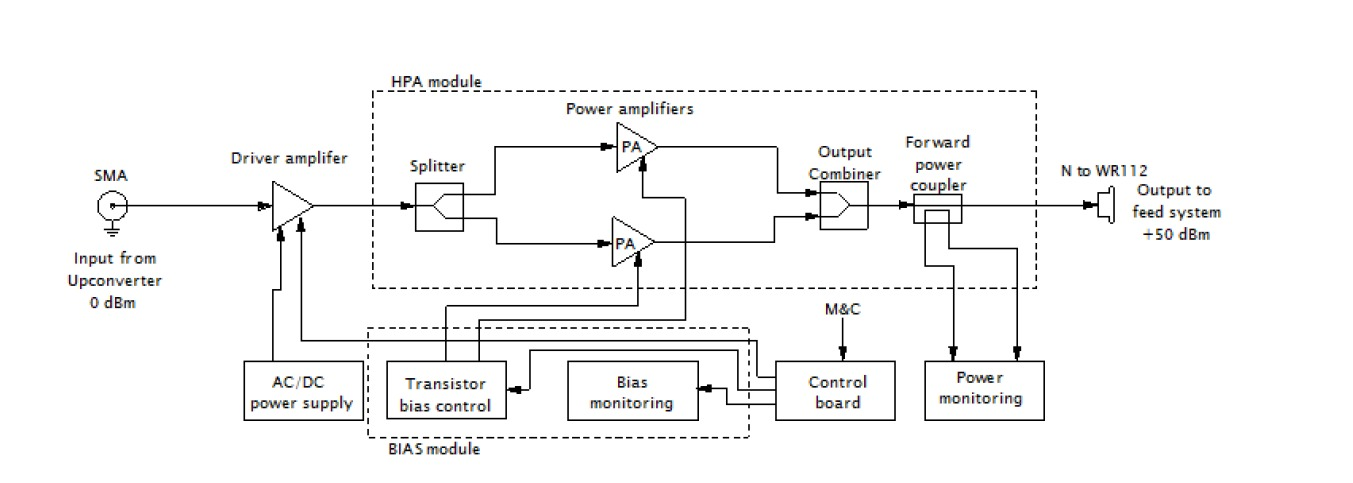
\includegraphics[width=0.9\textwidth]{pictures/HPA.jpg}\hspace{1cm}
    \caption{HPA vispārīga blokshēma \cite{bleideris2024xband}}
\end{figure}
1.3. att. var redzēt pašu jaudas pastiprinātāju ar ieejas filtriem. $V_{G}$ un $V_{D}$ ir pieslēgvietas, kuras ir jaudas pastiprinātāja vadībai un barošanas pievadei.
\begin{figure}[H]
	\centering
    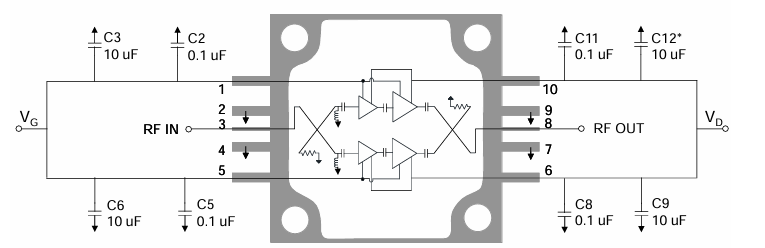
\includegraphics[width=0.9\textwidth]{pictures/pa.png}\hspace{1cm}
    \caption{QPM1017 sērijas RF jaudas pastiprinātājs}
\end{figure}
Šī darba ietvaros tiek izstrādāta darba punkta iestatīšana un atiestatīšanas sistēma, kas ir vadāma caur tīklu no kontroles datora, un jaudas monitoringa sistēma, kas mēra izstaroto un atstaroto jaudu.

%\section{Augstas jaudas RF pastiprinātājs}
Radiofrekvences \cite{poweramplifieroverview} (RF) tīkla signālu ķēdē jaudas pastiprinātāji ieņem vietu kā pēdējais elements, sekojot tādām komponentēm kā maztrokšņojoši pastiprinātāji (LNA), jaucējiem un citām signālu apstrādes pakāpēm. Jaudas pastiprinātāji ir atbildīgi par būtisku uzdevumu – pastiprināt signālu līdz nepieciešamajam jaudas līmenim tā raidīšanai. Signāls tiek pastiprināts, lai spētu pārraidīt signālu lielos attālumos.

RF jaudas pastiprinātāji ir sastopami gandrīz visās bezvadu ierīcēs – sākot no bezvadu komunikācijas sistēmām, satelītkomunikācijām, raidīšanas iekārtām, mobilajiem tālruņiem līdz IoT ierīcēm.

\section{Dziļā kosmosa tīkla spektra sadalījums}
DSN \cite{nasajplfreq} ir izstrādājis frekvenču sadalījuma kanālu plānus, lai ērti un pārskatāmi var apskatīt dziļās kosmosa misijas spektrālo sadalījumu (B kategorija, lielāka par 2 miljoniem km no Zemes) S, X un Ka joslām saskaņā ar SFCG ieteikumiem. Plāni pieļauj vienlaicīgu fāzes saskaņotu augšupsaiti (Zeme-kosmoss, \textit{Uplink}) un lejupsaites (kosmoss-Zeme,\textit{Downlink}) pārraides, kur augšupsaite un lejupsaite ir vienā vai dažādās joslās.\\
ITU piešķir un regulē frekvenču spektru gan komerciālām, gan valstiskām vajadzībām. ITU galvenais mērķis ir koordinēt telekomunikāciju tīklu un pakalpojumu darbību visā pasaulē, pārvaldīt radiofrekvenču spektra un satelīta orbītu sadali, kā arī veicināt piekļuvi ICT, lai atbalstītu ilgtspējīgu attīstību.\\
CCSDS ir starptautiska kosmosa aģentūru organizācija, kas izstrādā un koordinē standartus pārraidei un datu sistēmām, lai atbalstītu kosmosa pētniecību. NTIA, ASV Tirdzniecības departamenta aģentūra, ir izpildvaras galvenā iestāde vietējiem un starptautiskiem telekomunikāciju un informācijas tehnoloģiju jautājumiem. NTIA novērtējumu pamatā ir tehniskie un regulatīvie kritēriji efektīvas un koordinētas frekvenču spektra izmantošanas kosmosa misijām. Apakšējā tabula apskata esošo un apstiprināto frekvenču sadalījumu joslās, kas arī iedalāt pēc attāluma no zemes.

\begin{table}[H]
\centering
\captionsetup{singlelinecheck=off, justification=raggedleft}
\caption{Frekvenču sadalījums joslā}
\begin{tabular}{|c|c|c|c|c|}
\hline
\multirow{2}{*}{Josla} 
& \multicolumn{2}{c|}{\makecell{Dziļā kosmosa josla \\ (2 milijoniem km no zemes)}} 
& \multicolumn{2}{c|}{\makecell{Dziļā kosmosa josla \\ (pēc 2 milijoni km no zemes)}} \\ 
\cline{2-5}
& \makecell{Augšupsaite \\ "zeme-kosmoss"} % Uplink
& \makecell{Lejupsaite \\ "kosmoss-zeme"} % Downlink
& \makecell{Augšupsaite \\ "zeme-kosmoss"} % Uplink
& \makecell{Lejupsaite \\ "kosmoss-zeme"} % Downlink
\\ 
\hline
S josla & 2110-2120 & 2290-2300 & 2025-2110 & 2200-2290 \\ 
\hline
X josla & 7145-7190 & 8400-8450 & 7190-7235 & 8450-8500 \\ 
\hline
K josla & N/A & N/A & 22550-23150 & 25500-27000 \\ 
\hline
Ka josla & 34200-34700 & 31800-32300 & N/A & N/A \\
\hline
\end{tabular}
\end{table}

\section{Vadības bloka specifikācija}
Tehniskā specifikācija tika izvirzīta no VSRC puses, kas tika definēta no izstrādātā HPA. HPA pēdējās pakāpes jaudas pastiprinātāja darba punkta iestatīšanas parametri, sagaidāmā tīkla vadība un jaudas detektora mērīšanas diapazons.
\begin{itemize}
    \item Darba punkta iestatīšanas procedūra (\textit{ang.} Bias-Up procedure)
    \begin{itemize}
        \item Iestatīt jaudas pastiprinātājiem strāvas ierobežojumu uz 18 A, strāvas ierobežojumu uz aizvaru 200 mA.
        \item Iestatīt aizvara spriegumu − 5.0 V.
        \item Pievadīt 24 V spriegumu HPA no elektrobarošanas avota.
        \item Pieskaņot aizvara spriegumu, līdz tiek sasniegta 3 A noteces strāvu.
        \item Pievadīt RF signālu.
    \end{itemize}
    \item Darba punkta atiestatīšana procedūra (\textit{ang.} Bias-Down procedure)
    \begin{itemize}
        \item Samazināt aizvara spriegumu līdz -5 V.
        \item Jaizmēra caurplūstošā strāva caur jaudas pastiprinātāju, jābūt ~ 0 mA.
        \item Jāatvieno barošanas avotu no jaudas pastiprinātāja.
        \item Jāatvieno RF signālu.
    \end{itemize}
    \item Vadība caur tīklu
    \begin{itemize}
        \item TCP servers.
        \item Līdz 8 klientiem.
        \item IPv4.
        \item Jaudas pastiprinātāja un barošanas avota ieslēgšana vai izslēgšana.
        \item Parametru monitorēšana:
        \begin{itemize}
            \item Temperatūra. 
            \item Spriegumi HPA barošanas avotam un vadības signālam (aizvaram).
            \item Caurplūstoša strāva cauri HPA.
            \item Sistēmas stāvoklis.
        \end{itemize}
        \item Kļūdu paziņošana. 
    \end{itemize}
    \item Izstarotās un atstarotās jaudas noteikšana ar RMS RF jaudas detektoru mērīšanas diapazonā no -50 dBm līdz 0 dBm.
\end{itemize}


\section{Darba punkta nodrošināšanas sistēmas izstrāde}
Šajā nodaļā tiek aprakstīta izstrādes plates modifikācija un testēšana, izstrādātie līdzstrāvas sprieguma pārveidotāji, industriālā barošanas avota vadības, strāvas mērīšanas, ieslēgšanas/izslēgšanas elektriskā principiālā shēmas. Daļas, kas nodrošina darba punkta iestatīšanas/atiestatīšanas funkciju.
\subsection{Monitoringa izstrādes plates modifikācija un integrēšana}
Lai ātrāk iegūtu vēlamo rezultātu, tika iegādāta izstrādes plate ar izvēlēto monitorēšanas integrālo shēmu EVAL-AD7293 \cite{eval_board} ar AD piedāvātu vadības sistēmu EVAL-SDP-CB1Z \cite{eval_board_mcu}.
\begin{figure}[H]
	\centering
    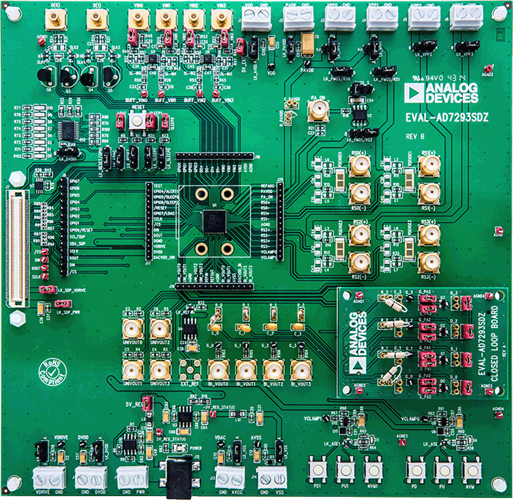
\includegraphics[width=0.5\textwidth]{pictures/EVAL-AD7293SDZ_TOP-web.png}\hspace{1cm}
    \caption{AD7293 izstrādes plate}
\end{figure}
\begin{figure}[H]
	\centering
    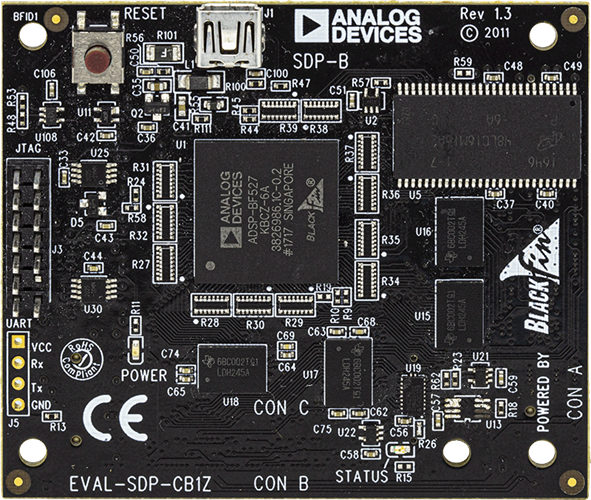
\includegraphics[width=0.5\textwidth]{pictures/EVAL-SDP-B-top-web.png}\hspace{1cm}
    \caption{Vadības sistēma monitorēšanas izstrādes platei}
\end{figure}
Šīs sistēmas pārbaudei tika izmantota AD lietojumprogramma, kas sniedz vispārīgu pārskatu par sistēmas funkcionalitāti.
\begin{figure}[H]
	\centering
    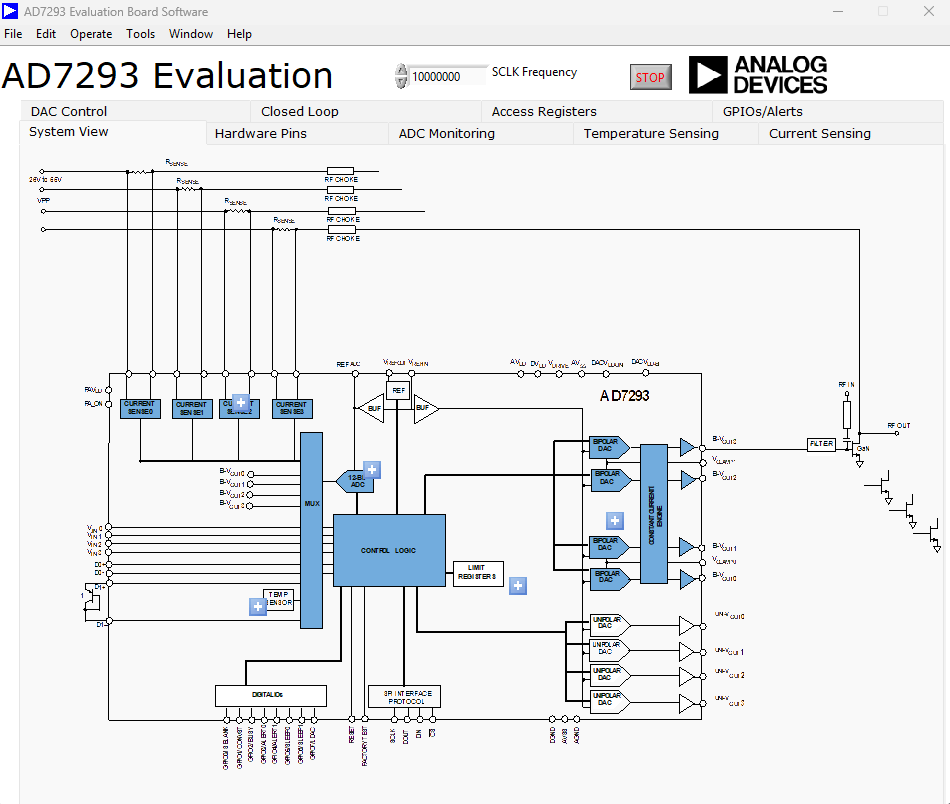
\includegraphics[width=0.6\textwidth]{pictures/eval-soft.png}\hspace{1cm}
    \caption{AD7293 testēšanas lietojumprogramma}
\end{figure}
Sekojot datu lapā pieejamai informācijai tika nodrošināta reģistru konfigurācijas secība un sasniegta vēlamā funkcionalitāte darba punkta iestatīšanai un atiestatīšanai.\\
Pēc nepieciešamās funkcionalitātes nodrošināšanas tika veiktas izstrādes plates modifikācijas - atlodēti SMA konektori, lai varētu pielodēt strāvas monitorēšanas sistēmas izvadus un ieslēgšanas/izslēgšanas sistēmas vadības izvadu, samainīti savienotājelementi, pievienoti barošanas avoti un pievienots digitālās loģikas analizators, lai monitorētu SPI saskarni.
\begin{figure}[H]
	\centering
    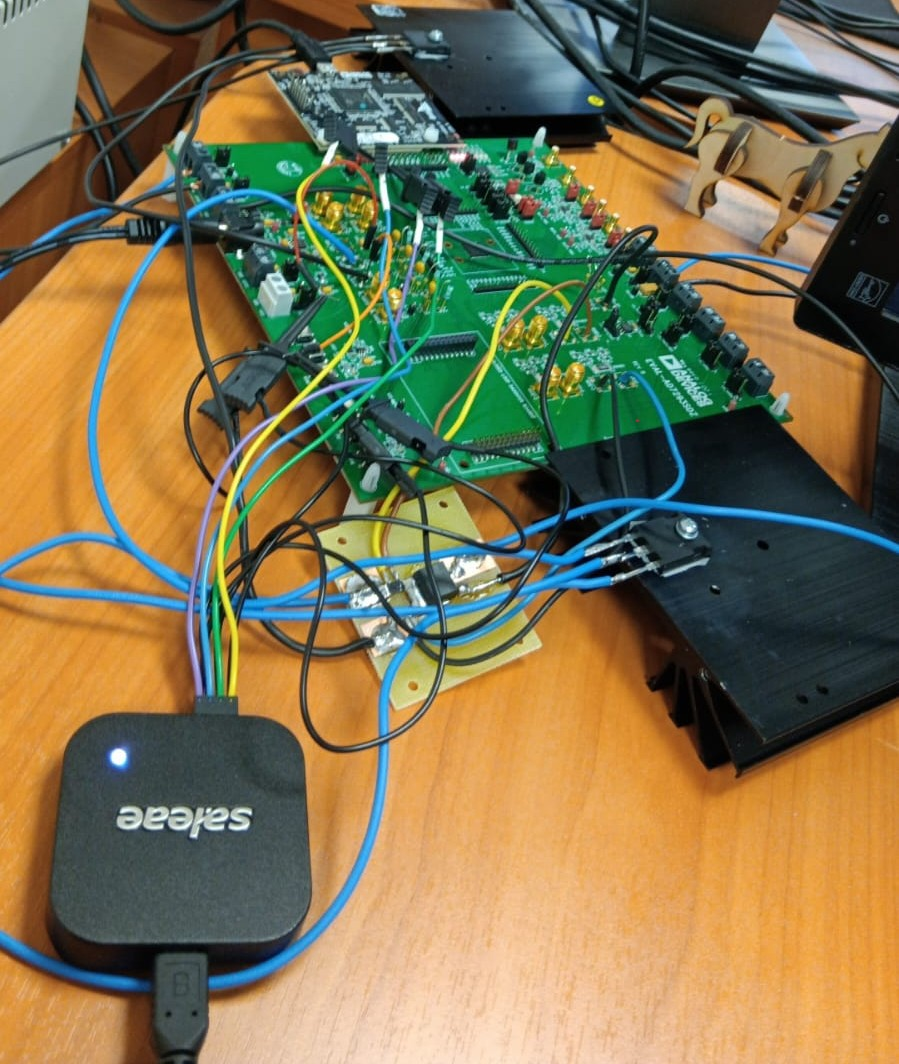
\includegraphics[width=0.5\textwidth]{pictures/daf.jpg}\hspace{1cm}
    \caption{Testa stends ar testa lauktranzistoriem}
\end{figure}
Tad tika sasniegts vēlamais rezultāts ar darba punkta iestatīšanu un atiestatīšanu.
\subsection{Sprieguma pārveidotāji, temperatūras sensora un 24 V barošanas avota vadības shēmas}
Tika izvēlēti lineārie sprieguma stabilizatori 5 un 9 V līnijām, neskatoties uz zemo efektivitāti, salīdzinot ar impulsa tipa sprieguma stabilizatoriem, tie nerada trokšņus izejā. Lineārie sprieguma stabilizatori tiek slēgti virknē, lai palielinātu 5 V regulātora efektivitāti, samazinot sprieguma kritumu uz tā. 12 V tiek pārveidots uz 9 V un no 9 V tiek pārveidots uz 5 V.  
\begin{figure}[H]
	\centering
    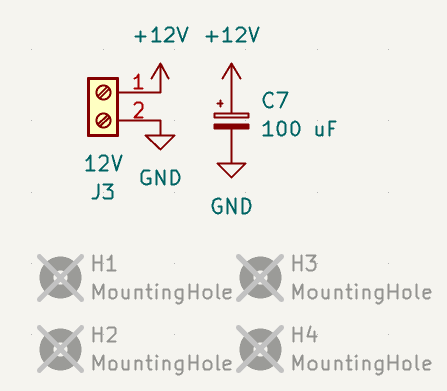
\includegraphics[width=0.6\textwidth]{pictures/inputs.png}\hspace{1cm}
    \caption{Ievadi, elektrolītiskais kondesators un urbjcaurumi}
\end{figure}
J3 terminālbloks ir paredzēts, lai varētu pieslēgt industriālo 12 V barošanas avotu. C7 elektrolītiskais kondensators paredzēts, lai mazinātu ieejas pulsācijas. H1, H2, H3 un H4 urbjcaurumi paredzēti, lai iespiedplati varētu iestiprināt korpusā.
\begin{figure}[H]
	\centering
    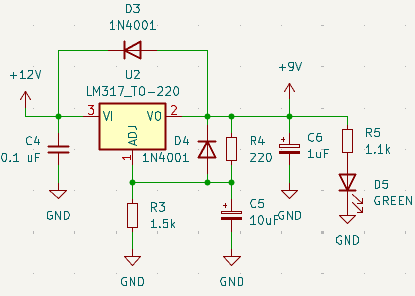
\includegraphics[width=0.6\textwidth]{pictures/9v.png}\hspace{1cm}
    \caption{12 V uz 9 V pārveidotais}
\end{figure}
\begin{figure}[H]
	\centering
    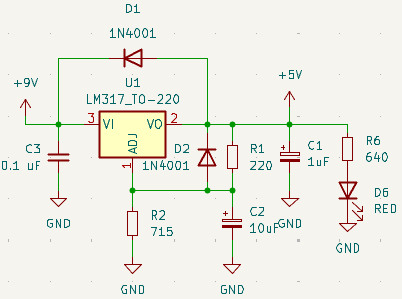
\includegraphics[width=0.6\textwidth]{pictures/5v.png}\hspace{1cm}
    \caption{9 V uz 5 V pārveidotais}
\end{figure}
Sprieguma iestatīšanai tiek izmantota atgriezeniskā saite, ko veido rezistori R1, R2, R3 un R4. Ķēdē tiek izmantoti keramiskie kondensatori C1, C3, C4 un C6. keramiskie un elektrolītiskie kondensatori ir vajadzīgi, lai mazinātu barošanas pulsācijas. R6 un R5 ir strāvas ierobežojošie rezistori D5 un D6 gaismas diodēm. D1, D2, D3 un D4 taisngriežu diodes paredzētas, lai neļautu C2 un C5 kondensatoriem izlādēties lineārā sprieguma izejā.
\begin{figure}[H]
	\centering
    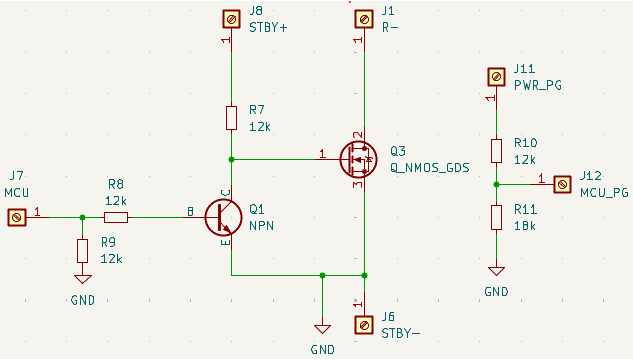
\includegraphics[width=0.6\textwidth]{pictures/24_control_detection.png}\hspace{1cm}
    \caption{24 V barošanas avota vadības sistēmu}
\end{figure}
J7 izvads paredzēts, lai varētu pieslēgt mikrokontrolliera vadības signālu. R8 ir paredzēts strāvas ierobežošanai NPN bipolārajam tranzistoram. R9 ir zema līmeņa piesaistes rezistors, lai pārejas procesā netiktu atvērts tranzistors. R7 rezistors ir paredzēts strāvas ierobežošanai un augsta signāla līmeņa piesaistei pie N kanāla lauktranzistora aizvara. J8, J1 un J6 izvadi paredzēti, lai varētu vadīt 24 V industriālo barošanas avotu. J11 ir paredzēts barošanas avota stāvokļa pieslēgvieta, kur R10 un R11 rezistori ir sprieguma dalītāji, lai varētu veikt sprieguma nolasi ar mikrokontrolliera.
\begin{figure}[H]
	\centering
    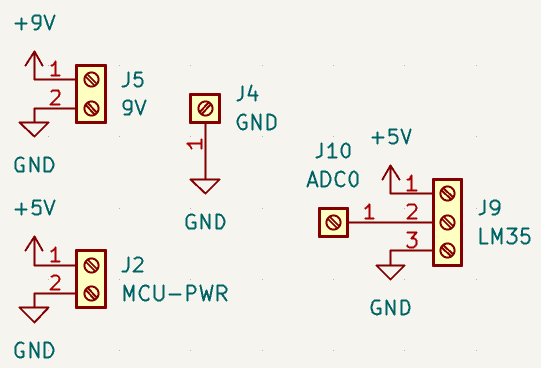
\includegraphics[width=0.6\textwidth]{pictures/outputs.png}\hspace{1cm}
    \caption{Pieslēgvietas MCU, temperatūras un patērētājiem}
\end{figure}
J5 un J2 terminālbloks paredzēts, lai varētu nodrošināt 9 V un 5 V barošanu patērētājiem. J9 terminālbloks paredzēts temperatūras sensora pieslēgšanai. J10 ir izvads, paredzēts mikrokontroliera ADC pieslēgvietai.
\begin{figure}[H]
	\centering
    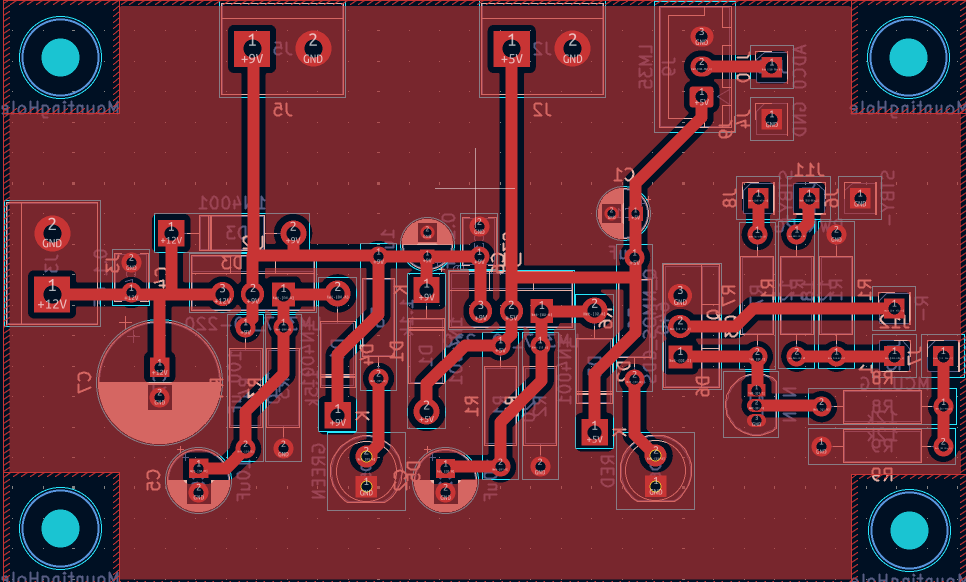
\includegraphics[width=0.6\textwidth]{pictures/power_board.png}\hspace{1cm}
    \caption{Iespiedplate lietojumprogrammatūrā "KiCad"}
\end{figure}
 Iespiedplate tika trasēta vienā slānī. Komponentes tika izvietotas pēc iespējas blīvāk, lai samazinātu iespiedplates izmērus. Tika izmantotas THT komponentes. Iespiedplate tika izfrēzēta ar augstskolā pieejamo frēzi.
\subsection{Strāvas mērīšanas iespiedplate ar ieslēgšanas/izslēgšanas slēdzi}
\begin{figure}[H]
	\centering
    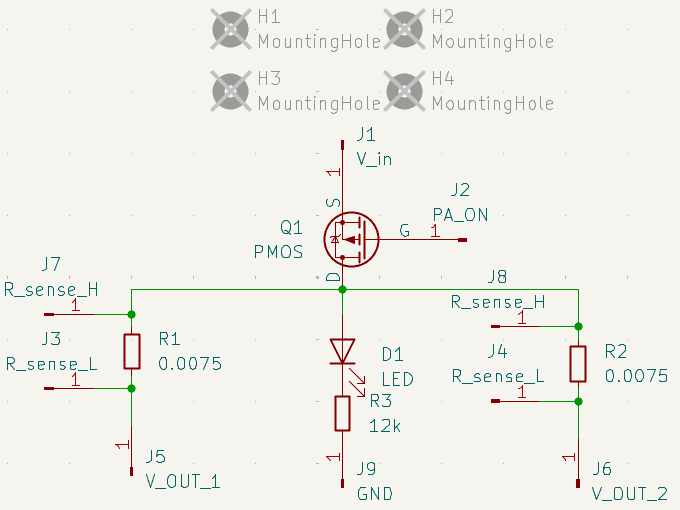
\includegraphics[width=0.6\textwidth]{pictures/shunt_resistors.png}\hspace{1cm}
    \caption{Strāvas mērīšanas shematiskais zīmējums}
\end{figure}
J1 terminālbloks ir 24 V pieslēgvietas nodrošināšanai. Q1 P kanāla lauktranzistors tiek izmantots slēdža režīmā, kas tiek kontrolēts ar AD7293 monitorēšanas integrālo shēmu, kas tiek pievadīts caur J2 termināli. R1 un R2 ir šunta rezistori strāvas mērīšanai. Šunta rezistori tika aprēķināti pēc izvēlētā mērīšanas diapazona AD7293 un maksimālās strāvas R <= 0.025/3 . J3, J4, J7 un J8 izvadi ir paredzēti, lai pieslēgtu strāvas mērīšanas sistēmu. D1 gaismas diodē ir paredzēta sistēmas stāvokļa identificēšanai. R3 rezistors ir paredzēts strāvas ierobežošanai, lai pasargātu gaismas diodi. J9 izvads paredzēts zemējuma nodrošināšanai.
\begin{figure}[H]
	\centering
    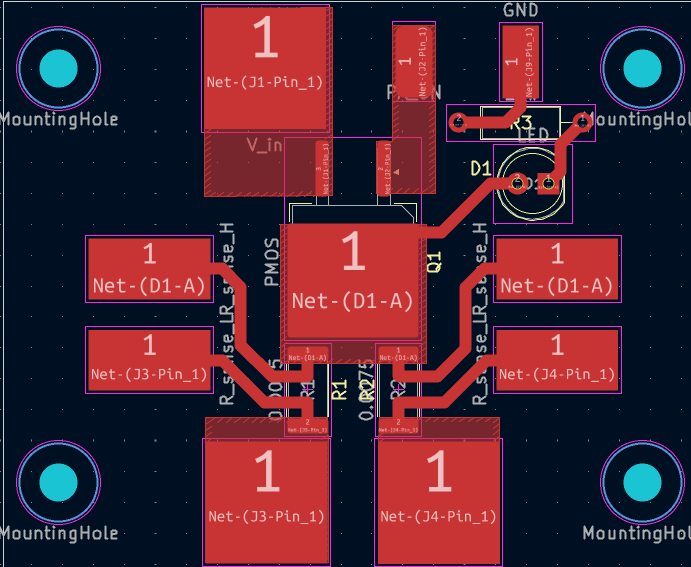
\includegraphics[width=0.6\textwidth]{pictures/shunt_resistors_board.png}\hspace{1cm}
    \caption{Iespiedplate lietojumprogrammatūrā "KiCad"}
\end{figure}
Tika izstrādāta vienslāņu plate ar blīvu komponenšu izvietojumu un attiecīgu jaudas celiņu platumiem. Tā tika izfrēzēta ar VeA pieejamo frēzi.

\section{Virzītais nozarotājs}
Virziena jaudas nozarotājs ir četru portu sistēma, kur viens ports ir izolēts no ieejas porta. Visi četri porti ideālā gadījumā ir salāgoti, un shēma ideālā gadījumā ir bez zudumiem. Nozarotāju var realizēt nesimetriskās un simetriskās mikroslokšņu līnijās, koaksiālajos kabeļos vai viļņvados. Tos visbiežāk izmanto signālu caurejošā signāla nolasei kā izstarotā un atstarotā jauda. Nozarotājā optimālā elektromagnētiskā saite starp līnijām tiek sasniegta, ja līniju sasaistītā posma garums ir vesels skaits ceturtdaļvilņu. Nozarotājs darbojās uz elektromagnētiskā principa, caurplūstošā strāva veido elektromagnētisko lauku, kas inducē strāvu izolētajā daļā, pārnesot signālu no viena atzara uz otru. Zemāk redzamais virziena atzarotājs ir izstrādāts X-joslas pastiprinātāja blokā, kur tiek piemeklēts risinājums vidējās jaudas mērīšanai.
\begin{figure}[H]
	\centering
    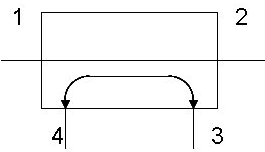
\includegraphics[width=0.9\textwidth]{pictures/bi-directional_coupler.png}\hspace{1cm}
    \caption{Atzarotāja elektriski principiālais apzīmējums}
\end{figure}

\section{Jauadas detektori}
Lieljaudas bezvadu sistēmas ir nepieciešams uzraudzīt un kontrolēt gan pārraidīto, gan saņemto RF jaudu \cite{rfpowerdetector}, kas tiek panākts ar RF detektoriem \cite{rfpowerdetector2}, kas tiek visbiežak izmantots bezvadu sistēmās, lai izstarotā jauda atbilstu signāla stipruma normatīvajām prasībām. Lai mērītu RF jaudu, tiek izmantotas trīs dažādas metodes: pīka detektors, logaritmiskais pastiprinātājs un RMS detektors. Katrai metodei tiek pielietota pēc sistēmas vajadzības. Lieljaudas pārraides sistēmās jauda tiek mērīta netiešā veidā, lai pēc iespējas mazāk ietekmētu sistēmu. RF jaudas mērīšanai neizmanto digitālas metodes, jo tās ir lēnākas nekā analogās metodes un ar augstāku jaudas patēriņu, lai sasniegtu līdzvērtīgu rezultātu. Logaritmiskais pastiprinātājs balstās uz diodes raksturīgo logaritmisko reakciju, kas rada izejas spriegumu, kas proporcionāls ieejas signāla jaudai, tāpēc tā izeja ir lineāra attiecībā pret ieeju decibelos. To plaši izmanto, īpaši gadījumos, ja signālam ir plašs dinamiskais diapazons. Tāpēc logaritmiskais pastiprinātājs tiek izmantots sistēmās ar impulsu signāliem, kā radariem. RMS detektors ģenerē spriegumu, kas proporcionāls signāla jaudas RMS vērtībai. RMS detektors ir piemērots signāliem ar augstu signāla amplitūdas pīķa-vidējās vērtības attiecību (crest-factor). Raidītāji ar amplitūdas pīķa-vidējās vērtības attiecību (10-15 dB) kļūst arvien izplatītāki, jo tiek plašāk izmantotas modernas modulācijas metodes, piemēram, augstākas kārtas QAM, CDMA sistēmās vai OFDM. 

Tā kā satelītkomunikācijām tiek izmantota augsta amplitūdas pīķa-vidējās vērtības attiecība modulācija, tiek izvēlēts RMS detektors kā jaudas mērīšanas risinājums.

\subsection{Apskatītie risinājumi}

LTC5582\cite{ltc5582} ir RMS jaudas detektors, kas darbojas frekvenču diapazonā no 40 MHz līdz 10 GHz un ar plašu mērīšanas diapazonu 62 dB. Tas darbojas frekvenču diapazonā no 10 MHz līdz 10 GHz un var apstrādāt ieejas signālus no –60 dBm līdz +2 dBm ar dažādiem amplitūdas pīķa-vidējās vērtības attiecībām.

ADL5906\cite{adl5906} ir RMS jaudas detektors, kas darbojas frekvenču diapazonā no 10 MHz līdz 10 GHz un ar plašu mērīšanas diapazonu 67 dB. Tas darbojas frekvenču diapazonā no 10 MHz līdz 10 GHz un var apstrādāt ieejas signālus no –65 dBm līdz +8 dBm ar dažādiem amplitūdas pīķa-vidējās vērtības attiecībām un joslas platumiem. Piedāvāta temperatūras stabilitāte plašā temperatūras diapazonā (no –55°C līdz +125°C). Nepieciešams 5 V barošanas avots un darba strāva ir 68 mA pie 25°C temperatūrās.

LTC5587\cite{ltc5587id} ir  RMS jaudas detektors ar integrētu 12 bitu seriālo ADC, kas darbojas frekvenču diapazonā no 10 MHz līdz 6 GHz. Mērīšanas diapazons ir no –34 dBm līdz 6 dBm. Detektora seriālā digitālā izeja nodrošina 12 bitu skaitlisko vērtību, kas tieši proporcionāla RF signāla jaudai dBm vienībās.

ADL5500\cite{adl5500} ir RMS jaudas detektors, kas darbojas no 100 MHz līdz 6 GHz. Nodrošina teicamu temperatūras stabilitāti ar gandrīz 0 dB mērījumu kļūdu visā temperatūras diapazonā. Nav plašs mērīšanas diapazons no -25 dB līdz 10 dB.

Tika izvēlēts ADL5906 jaudas detektors, jo piedāvā visplašāko mērīšanas diapozonu no -65 dBm līdz +8 dBm ar temperatūras kompensēšanas shēmu. Frekvenču diapozons atbilst X-joslai, kā arī paredzēts ar modulētiem signāliem ar lielu amplitūdas pīķa-vidējās vērtības attiecību un joslas platumu.
\section{Differenciālā mērīšanas metode}

Lielākā daļa osciloskopu \cite{tiepie_diffmes} ir viena ieejas puse vienmēr ir savienota ar zemi, bet otra puse ar interesējošo punktu elektriskajā ķēdē.
\begin{figure}[H]
	\centering
    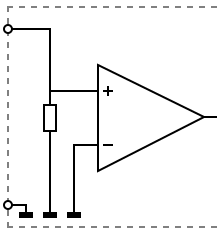
\includegraphics[width=0.5\textwidth]{pictures/osc_1_probe.png}\hspace{1cm}
    \caption{Osciloskopa izvada struktūra}
\end{figure}

Tāpēc spriegums, ko mēra ar osciloskopu, vienmēr tiek mērīts starp konkrēto punktu un zemi. Kad mērāmā ķēde ir savienota ar to pašu references punktu, tad var izveidoties īssavienojums, kas var sabojāt ķēdes daļu un osciloskopu. Lai no tā izvairītos, tiek mērīti vēlamie elektriskie ķēdes posmi ar differenciālo metodi. Šī metode aprēķina sprieguma starpību starp diviem punktiem. Lielākajā daļā osciloskopu to var izdarīt, savienojot vienu no kanāliem ar vienu punktu un otru kanālu ar otru punktu un pēc tam izmantojot osciloskopa matemātisko funkciju Ch1 - Ch2, lai parādītu faktisko sprieguma starpību.
\begin{figure}[H]
	\centering
    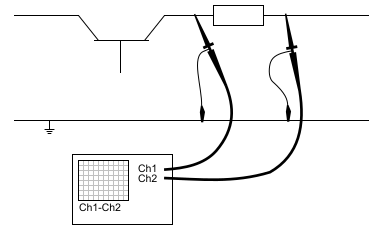
\includegraphics[width=0.5\textwidth]{pictures/osc_2_diff.png}\hspace{1cm}
    \caption{Differenciāla mērīšana izmantojot osciloskopu}
\end{figure}

\section{S-parametri}
Izkliedēšanas parametri \cite{s_param} (S-parametri) tie raksturo, cik liela signāla daļa tiek atstarota, izplatīta caur vai pārnesta starp ķēdes portiem. Signāla parametri S ir kompleksi lielumi, kas ietver gan amplitūdas, gan fāzes raksturlielumus. Elektriskā ķēde ir ierīce ar vienu vai vairākiem portiem, kur katrs ports var pārraidīt, absorbēt vai atstarot RF signālu. 
Elektriskā ķēde tiek klasificēta pēc portu skaita: 
\begin{itemize}
    \item Viens ports: piemēram, ir antena vai 50 omu slodze.
    \item Divi porti: piemēram, ir filtrs vai pastiprinātājs.
    \item Trīs porti: piemēram, ir virziena atzarotājs.
\end{itemize}
Ķēdes analizē, ievadot RF signālu noteiktā portā un mērot RF līmeni, kas parādās šajā portā (atstarotais signāls) un/vai citos portos. Parasti vienlaikus tiek ievadīts tikai viens signāls vienā portā, un mērījumi tiek veikti dažādu frekvenču diapazonā. Ierīci, ko parasti izmanto ķēdes analīzei, sauc par ķēžu analizatoru.
S parametru apzīmē ar burtu “S”, kam seko divi apakšraksti, kur pirmais apakšindekss norāda izejas portu, bet otrais apakšindekss ieejas portu. Piemēram:
\begin{itemize}
    \item Ja signāls tiek pievadīts portā 1 un izmērīts porta 1, tad S-parametru apzīmē kā $S_{11}$.
    \item Ja signāls tiek pievadīts portā 1 un izmērīts porta 2, tad S-parametru apzīmē kā $S_{21}$.
    \item Ja signāls tiek pievadīts portā 2 un izmērīts porta 3, tad S-parametru apzīmē kā $S_{32}$ u.t.t.
\end{itemize}
\begin{figure}[H]
	\centering
    \includesvg[width=0.6\textwidth]{pictures/s-param_diag.svg}
    \hspace{1cm}
    \caption{S-parametru nosaukumu diagramma}
\end{figure}
Divu portu elektriskā ķēde ir aprakstīta ar četriem S parametriem:
\begin{itemize}
    \item $S_{11}$/$S_{22}$ ir ieejas atstarošanas koeficients. Tas mēra ieejas signāla daļu pie 1. porta, kas tiek atstarota atpakaļ pie 1. porta. Šis parameters norāda, cik liela daļa no ieejas signāla tiek atstarota saistībā ar impedances nesakritību.
    \item $S_{21}$/$S_{12}$ ir pārvades koeficienti. Tas mēra ieejas signāla daļu pie 1. porta, kas tiek pārraidīta uz 2. portu. Šis parameters norāda signāla pārraides efektivitāti no ieejas uz izeju.
\end{itemize}

\begin{figure}[H]
	\centering
    \includesvg[width=0.6\textwidth]{pictures/s_param_2_port.svg}
    \hspace{1cm}
    \caption{2 portu s-parametru diagramma}
\end{figure}
S parametrus var attēlot kā N×N matricu, kur N ir portu skaits tīklā. Katrs matricas elements $S_{xy}$ apzīmē izkliedes parametrus no porta y uz portu x. To var reprezentēt šādi:
\[
\mathbf{S} = \begin{bmatrix}
  S_{11} & S_{12} \\
  S_{21} & S_{22}
\end{bmatrix}
\]
